

\chapter[Prior impropriety]{Appendix A} \label{AppendixA}

The penalty matrix $\mathbf{P}$ corresponding to an undirected $RW_\kappa$ prior over parameter vector $\lambda \in \mathbb{R}^C$ has rank $C - \kappa$ and the resulting matrix $\Sigma^{-1} = \mathbf{Q} = \mathbf{P}/\tau^2$ is not a valid precision matrix. In the $RW_1$ case this can be mitigated by jittering the elements of $\mathbf{P}$. For $\kappa > 1$ a possibility is to estimate only $C - \kappa$ of the $C$ parameters in $\lambda$,  from which the remaining $\kappa$ so-called {\it pinned} parameters (each of which has a conditional variance of zero) can be computed following the properties of the multivariate normal distribution. This strategy amounts to  constraining the relevant linear combinations to have zero variance, from which a proper prior on a lower dimensional subspace is obtained \shortcite{paciorek_2009, rue_gaussian_2005}. 

Another possibility is to estimate the autoregressive parameter $\omega$ mentioned in \ref{penalty_matrix} (see footnote~\ref{footnote_car}), which results in a proper prior. \citeA<See>{paciorek_2009} \citeA<and>{banerjee_hierarchical_2004} for potential drawbacks to this approach.

An entirely different tactic would be to estimate an arbitrary tridiagonal precision matrix rather than specifying the penalty matrix and estimating the hierarchical variance/precision parameter. One way to do this would be to decompose the precision matrix into conditional correlations and standard deviations. This is possible to do in Stan and should be explored in future work to sidestep the matrix singularity problems. 


\clearpage
\chapter[Seats-votes curves]{Appendix B}\label{AppendixB}

Seats-votes curves for various values of $\rho$ and $\lambda$. On the top $\lambda$ is fixed at 0, while below $\rho$ is fixed at 1.


\begin{figure}[h]
\centering
	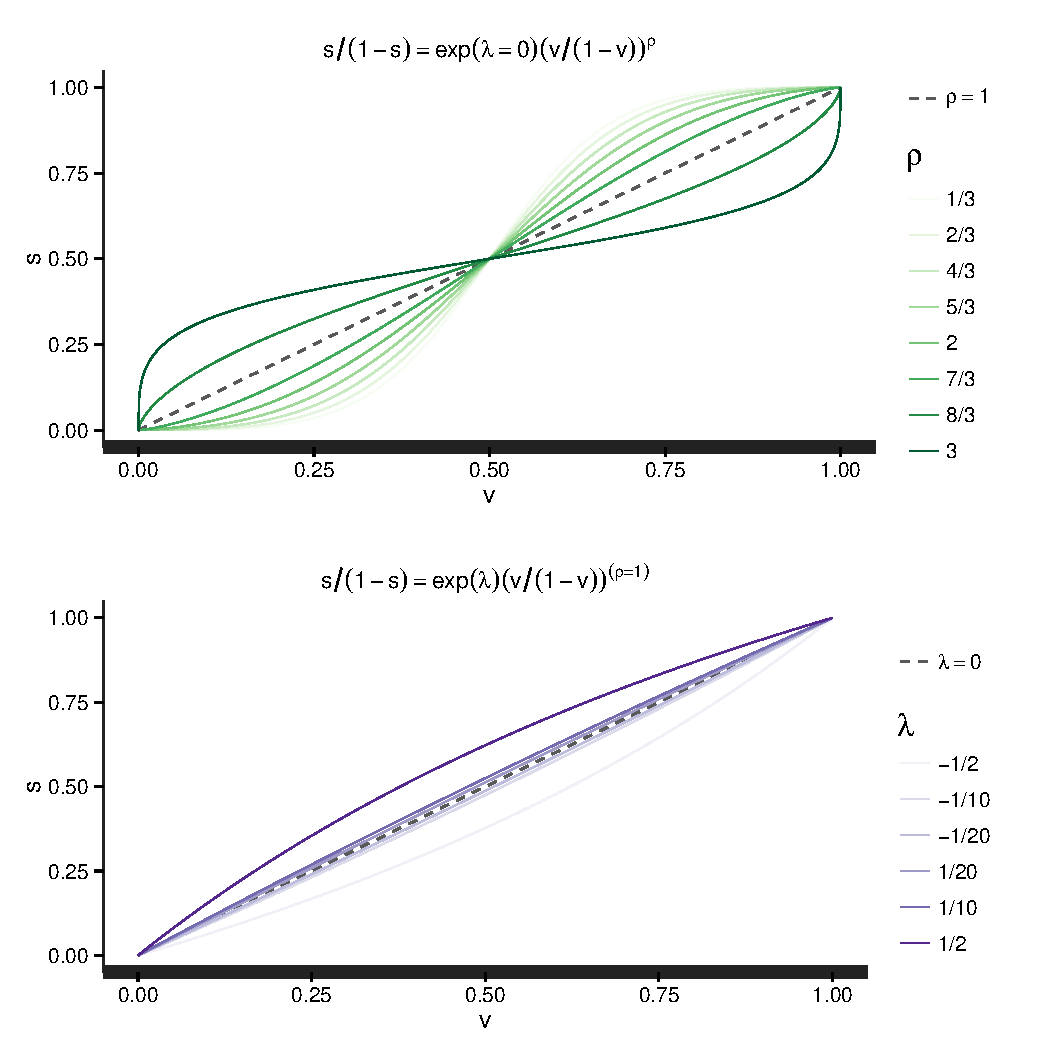
\includegraphics[scale=0.75]{sections/figs/seats_votes}
\label{fig:seats_votes}
\end{figure}